\section{Sokoban Solver}
This part of the report will, as suggested by the title, present the sokoban solver.
Initially, a brief overview of the various iterations of the method used to solve the problem will be presented, after which the final solution is shown in more detail.
During the process a few optimizations were done to reduce the computational workload of the solver.

\subsection{The Sokoban Map}
A sokoban map consists of walls, goals, diamonds and the man. 
Each of these are represented using simple symbols and characters.
The man is represented by 'M' or 'm' when standing on a goal. 
A diamond is represented by 'J' or 'j' when standing on a goal.
A goal is represented by 'G' and a wall by 'X'.
When necessary, deadlock situations will be represented by a red square while non-deadlocks will have a green square.

\subsection{The Algorithm and A*}
A*, being a well-established algorithm for pathfinding problems is an obvious candidate for creating the solver.
The solver was developed mostly using \cite{stanford} as reference.
A* is a greedy algorithm that, when given an appropriate, underestimating heuristic, is guaranteed to find the shortest path in terms of whatever cost described by the heuristic.
In order to use the algorithm, it is necessary to define the terms used by the algorithm:

\paragraph{State:}
First, it is necessary to define what constitutes a state. 
Any state should be uniquely distinguishable from any other state and should hold the information necessary to describe the goal condition.
In the case of the sokoban solver, the position of the diamonds and the man on the map and the map itself describes a state.
However, it is unnecessary to include the map in the state representation as this is static.
Theoretically, one could leave out the position of the man as well as this is irrelevant when describing the goal condition.
It was chosen to include the position of the man in the state for ease of access in various parts of the implementation.

\paragraph{Initial State:}
\label{sec:initialstate}
This is the starting point of the algorithm. 
In the case of the competition map, see figure \ref{fig:competitionmap}, the state is defined as follows:

\begin{figure}
	\centering
	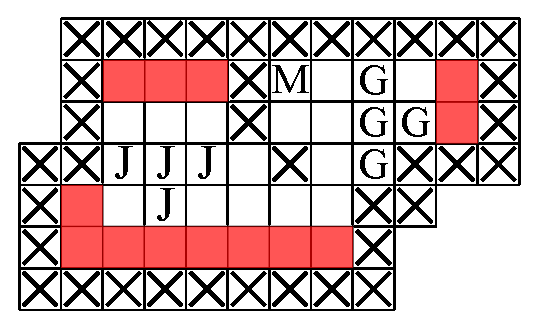
\includegraphics[width=.75\linewidth]{images/competitionmap}
	\caption{The sokoban map used at the competition.}
	\label{fig:competitionmap}
\end{figure}

\begin{lstlisting}
	Man: {1,6}
	Diamonds: {3,2;3,3;3,4;4,3}
\end{lstlisting}

\paragraph{Goal State:}
This is the state such that, when reached, the problem is solved. 
Upon each iteration of the algorithm each new state is compared to this one in order to decide whether another iteration should be done.
It is worth noting that the position of the man is disregarded when comparing with the goal state as the man has no impact on the win condition of the game.
Additionally, the order of the diamonds is irrelevant.
For the competition map the goal state is defined as:

\begin{lstlisting}
	Man: {0,0}
	Diamonds: {1,8;2,7;2,8;3,8}
\end{lstlisting}

\paragraph{Heuristic:}
The heuristic is the measure by which the algorithm determines which state to treat next.
It should provide a measure of the approximated distance to the goal condition. 
This is done by applying the wavefront algorithm to the map with goals as the initial nodes.
The heuristic is then just $\sum_{i}$wf(Diamonds[i]) where i goes from zero to the number of diamonds.
Using this method means that the heuristic will reflect the distance from each diamond to the goal closest to the diamond. 
This ensures that the heuristic is underestimated, as is required to guarantee the "shortest path" property of A*.
Initially it was considered to add a penalty to switching diamonds, thereby encouraging the algorithm to finish work on one diamond before starting the next.
This approach was thought to result in a more, subjectively, "natural" looking solution of the map.
It was eventually abandoned due to unnecessity and a desire for simplifying the code base.

\paragraph{Cost:}
This is the exact cost of going from the initial state to some state $S_i$. 
In this case this cost is defined simply as the number of steps the man must take in order to reach $S_i$.\\~\\

The parts described above are connected in the \texttt{solve()} function. 
This function holds the implementation of the A*.
It holds the two sets, \texttt{open} and \texttt{closed}.
\texttt{open} should always be sorted such that the state with the lowest heuristic is the first element.
This makes the \texttt{priority\_queue} a good candidate as the PQ allows for simple sorting of the set.
\texttt{closed} should be searched for every new state to ensure that they have not been attempted previously, before being pushed onto \texttt{open}.
In order to easily search for a state \texttt{map} is used. 
A string is used for hashing. It contains the diamond and man positions and is generated from a state. 
The initial state mentioned previously would produce \texttt{"3233344316"}.\\
The implementation used does allow for some optimization;
Since the order of the diamonds does not uniquely identify one state, by changing the hashing function such that it compares every diamond position in a state, with every position in the string, the number of states pushed onto \texttt{open} could potentially be reduced.\\
When a state is taken from \texttt{open} all of its potential children are found using \texttt{get\_children()}. 
This function utilizes the wavefront algorithm as well.
By applying a wavefront with the diamonds set as walls and the man as the initiator, every reachable position will have a value $>1$.
Every side of each diamond is then checked, first to see if the man can reach that side, then to see if the opposite side of the diamond is a valid new position for the diamond.
If both return true that state is created and saved.

\subsection{Deadlock Detection}
To enhance the solving speed of the sokoban solver a preprocessing scheme named deadlock detection is applied to the map before solving.
A deadlock is a position on that a diamond can be pushed to, but not retrieved from, making it impossible to solve the puzzle. 
Applying deadlock detection reduces the search space and thereby also the search time.
A deadlock can occur at corners or along edges between two corners and as such the detection scheme will start by finding corners in the map.
See figures \ref{fig:deadlockcorner} and \ref{fig:deadlockedge}.
%image
% Different Deadlock  situations
%	Corner
%	edge
Corners are found by inspecting the neighbouring map position. 
If the current position is (i,j) and the element at that position is '.' then four situations are inspected, one for each possible corner. 
If the position before, (i-1,j), above, (i,j-1), and the diagonal, (i-1,j-1), all have element 'X', then (i,j) is an upper left corner. 
Similar situations exist for the remaining three corners.
Any corner found will be marked 'D' on the map.
% image
%	 up-Left corner 
% 	 up-right corner
%  down-left corner
%  down-right corner

\begin{figure}[H]
    \centering
    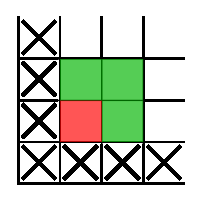
\includegraphics[width=0.40\textwidth]{images/deadlock_corner_leftup}
    \caption{Lower left corner.}
    \label{fig:deadlockcorner}
\end{figure}

when all corners on the map are found they are compared to see if they are part of the same edge.
This is done by taking corners that share the same row or column value and then traversing the map along either the row or column (depending on which they had in common). 
If, when traversing, a diamond or goal is met, the edge will not be deadlocked.
If the other goal is reached, the edge is deadlocked.
In order to avoid creating a deadlock in the situation in figure \ref{fig:deadlockopposite}, while traversing, each neighbouring position is checked, if non of the four neighbours have element 'X', the traverse is terminated.

%
% Traversing edge

\begin{figure}[H]
    \centering
    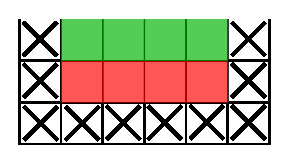
\includegraphics[width=0.40\textwidth]{images/deadlock_edge}
    \caption{Deadlocked edge between two corners}
   	\label{fig:deadlockedge}
\end{figure}
 
 % Traversing edge
 %  dont create a wall
 \begin{figure}[H]
	\centering
    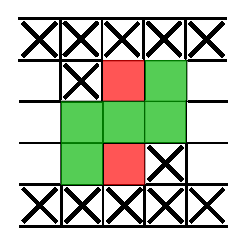
\includegraphics[width=0.40\textwidth]{images/deadlock_opposite}
    \caption{Traversing edge could create a wall here. }
	\label{fig:deadlockopposite}
\end{figure}
  
Applying deadlock detection to the competition map has shown great improvement not only for solving speed, but also on the memory usage of the solver. 
The lower memory usage is caused by the reduced number of children in the \texttt{open} and \texttt{closed} lists.
Search time is reduced significantly since there are fewer children to search through. 
Figure \ref{fig:test} shows the improvement of both time and memory when using deadlock detection versus not using deadlock detection.
It was found that the solver ran for approximately 471.6 s without deadlock detection and for 61.2 s with deadlock detection. 
This is a x \% improvement.
As for memory the usage was mostly halved at 392.6Kb with deadlock detection and 749Kb without deadlock detection.
 
 \begin{figure}[H]
\centering
\begin{subfigure}{.5\textwidth}
  \centering
  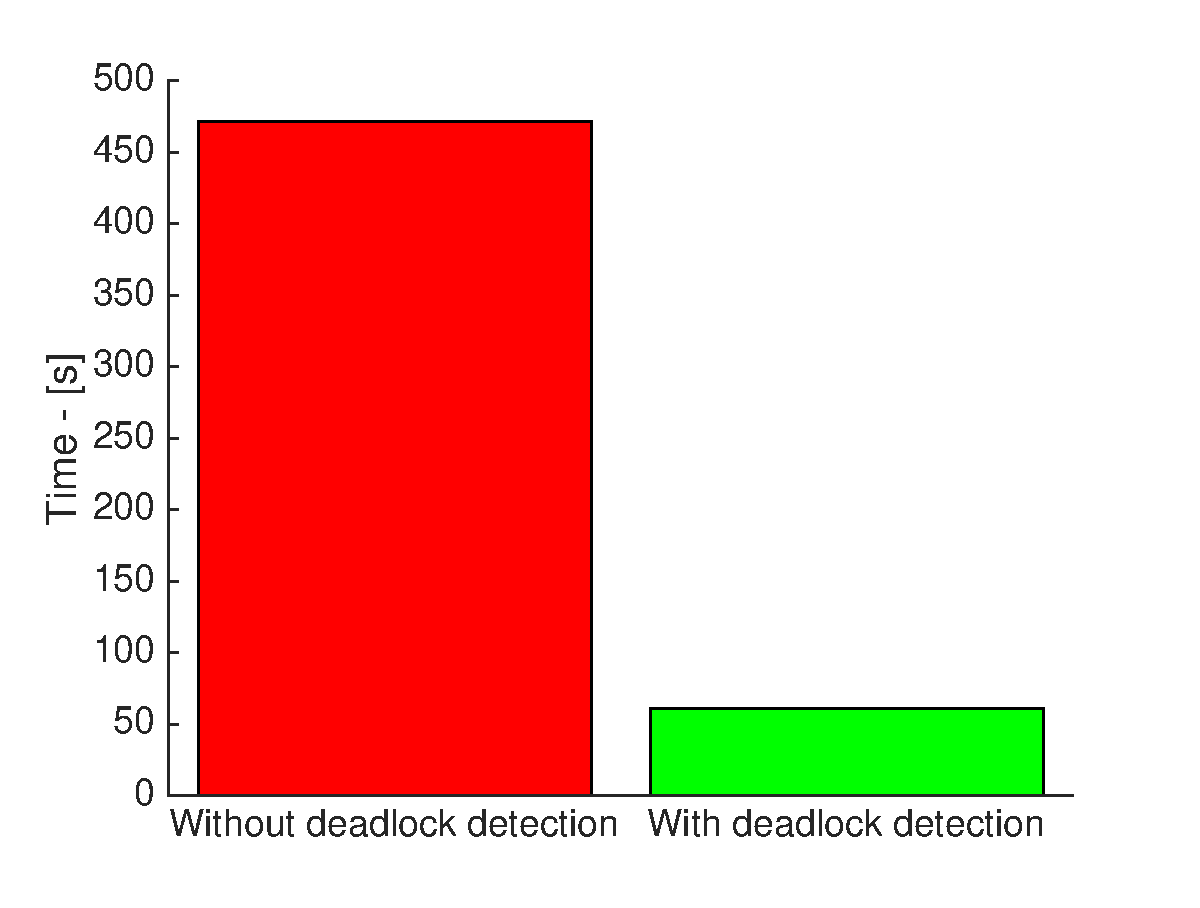
\includegraphics[width=0.98\linewidth]{images/deadlockImprovement}
  \caption{Time improvement}
  \label{fig:sub1}
\end{subfigure}%
\begin{subfigure}{.5\textwidth}
  \centering
  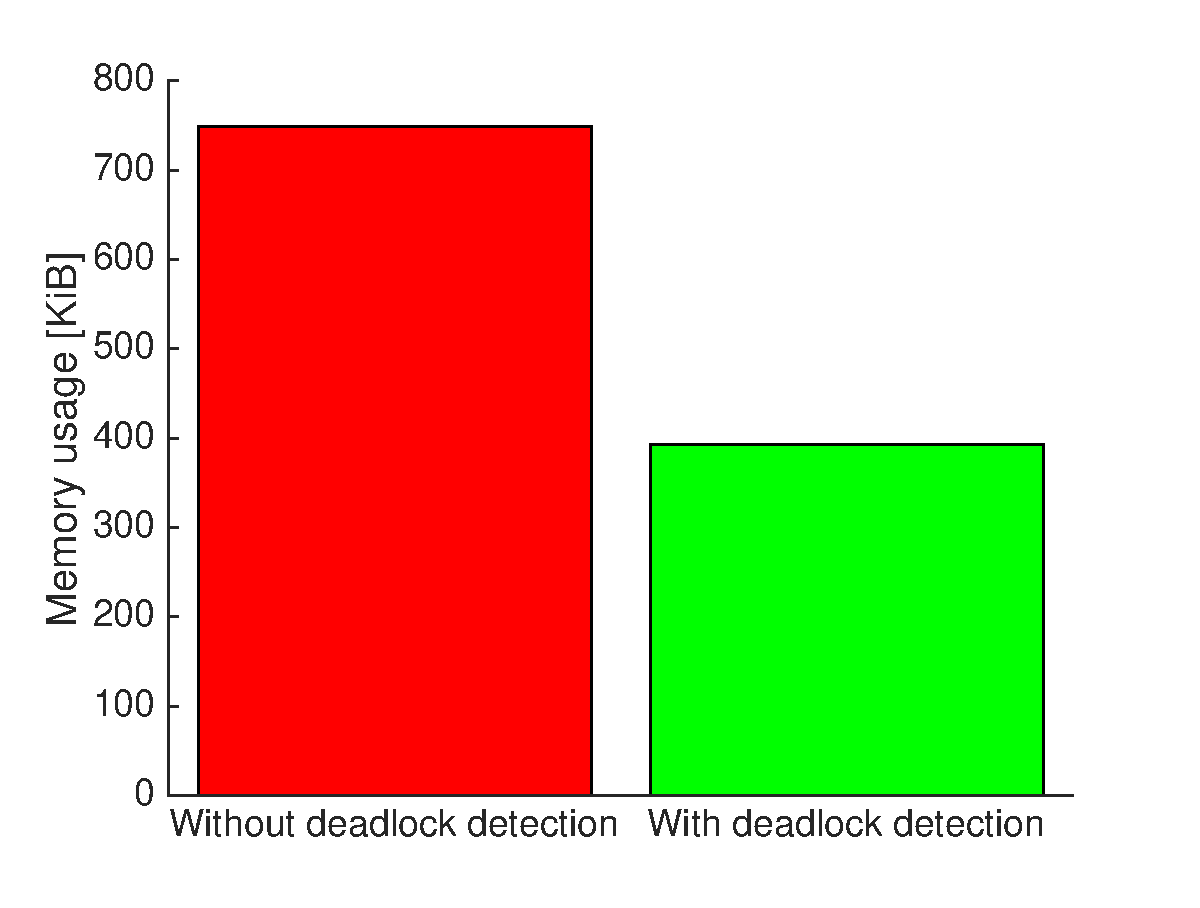
\includegraphics[width=0.99\linewidth]{images/Memory_usage_1}
  \caption{Memory usage improvement}
  \label{fig:sub2}
\end{subfigure}
\caption{Performance of the sokoban solver when applying deadlock detection (green) vs not applying deadlock detection (red).}
\label{fig:test}
\end{figure}
 
An additional possible optimization could be the use of an online deadlock detection method.
This method would be applied each time a new child is considered, if it contains a deadlocked state, it can be immediately removed.
Such a state can occur if four diamonds are pushed such that they form a square.
Furthermore, the diamonds can create new deadlocks in combination with parts of the map.
 
% Online deadlock detection
% J J
% J J J 
% J J J J
% J J J J 
 
% J
% J

% J
% J
% J

% J
% J
% J
% J
Based on the performance gain of the offline method, expanding the deadlock detection to an online scheme as well, might prove beneficial.
However, the problem with doing this form of deadlock detection itself, is that new, map specific and undefined deadlock cases would most likely keep appearing, and therefore making a complete deadlock detection tedious at best, impossible at worst.
Additionally, checking for a large variety of different deadlocks in the brute force manner as has been done here, may add an unacceptably large extra computation to generating a new child.
Something that happens a significant number of times throughout running the solver.

\subsection{Memory Leaks}
At a point during the development process the solver was capable of solving simple maps but quickly filled the memory of any computer on larger maps. Eventually the conclusion was drawn that a memory leak was present.
In order to help track down the origin of the memory leak a heap profiler was used. Specifically Massif \cite{massif}.
Massif provides detailed information about the heap used by the program.
One drawback of massif is that it greatly increases the time required to run the program.
Due to this inconvenience, the memory leak debugging was done using a simpler map, as seen in figure \ref{fig:simplemap}.

\begin{figure}
	\begin{subfigure}[t]{.49\linewidth}
		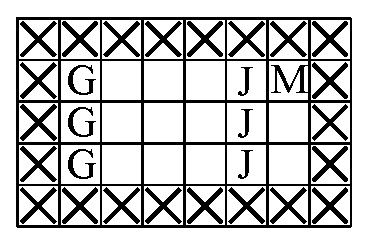
\includegraphics[width=\linewidth]{images/memorymap}
		\caption{Simple map used while debugging.}
		\label{fig:simplemap}
	\end{subfigure}
	\begin{subfigure}[t]{.49\linewidth}
		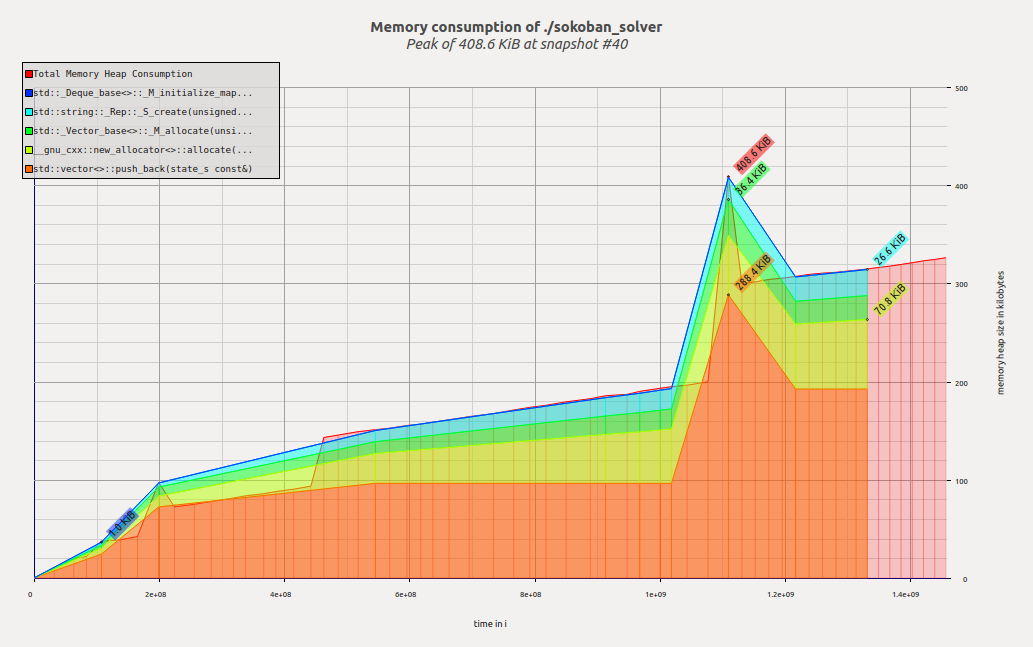
\includegraphics[width=\linewidth]{images/massif_small}
		\caption{The output from Massif when analysing the heap of the sokoban solver.}
		\label{fig:simplemassif}
	\end{subfigure}
\end{figure}

The resulting graph when solving the simple map using massif can be seen in figure \ref{fig:simplemassif}.
Each colour represents the memory usage of a specific function, with the most memory intensive function being the lowest on the graph.
By examining these graphs it was possible to find the function causing the memory leak, namely, the wavefront function.
With the liberal use of wavefronts throughout this implementation of a sokoban solver, it is no surprise that a memory leak here would cause significant issues.
By removing this leak it was possible to go from using 6 Gb of ram and an equal amount of swap and getting no solution, to using only 64.9 Mb of memory and producing a solution within a minute.
A slight improvement.